% ICLR 2026 submission — first draft.
% Replace the article preamble with `\documentclass{iclr2026_conference}` once
% the official style file is in this directory; the rest of the body is
% conference-agnostic.
\documentclass[10pt,letterpaper]{article}

\usepackage[margin=1in]{geometry}
\usepackage[utf8]{inputenc}
\usepackage[T1]{fontenc}
\usepackage{lmodern}
\usepackage{microtype}
\usepackage{graphicx}
\usepackage{tikz}
\usetikzlibrary{arrows.meta,positioning,fit,backgrounds,shapes.geometric}
\usepackage{booktabs}
\usepackage{multirow}
\usepackage{array}
\usepackage{caption}
\usepackage{subcaption}
\usepackage{amsmath,amssymb}
\usepackage{xcolor}
\usepackage{hyperref}
\usepackage{url}
\usepackage{authblk}
\usepackage{enumitem}
\usepackage{algorithm}
\usepackage{algpseudocode}
\usepackage[round,authoryear]{natbib}
\bibliographystyle{plainnat}

\graphicspath{{../results/consolidated_analysis/}{../results/consolidated_analysis/plots/}{../results/consolidated_analysis/commitment_locus/}{../results/consolidated_analysis/missed_confounder/}}

\hypersetup{
  colorlinks=true,
  linkcolor=blue!60!black,
  citecolor=blue!60!black,
  urlcolor=blue!60!black
}

\title{\textbf{When Should an LLM Search?\\
A Calibration-Centric Evaluation of Search Behavior and a Hidden Generalization Gap Under Natural Paraphrases}}

\author{Anonymous Authors}
\affil{Paper under double-blind review at ICLR 2026}

\date{}

\begin{document}
\maketitle

\begin{abstract}
Modern LLMs deployed as info-seeking assistants must decide, on the fly, whether to
lean on their parameters or reach out to a live web search. As both parametric
knowledge and agentic tool use grow, the right interplay between recall and retrieval
becomes genuinely unclear --- yet existing evaluations measure end-task accuracy and
question-level tool use, never asking the upstream question: \emph{given that a model
can search, does it search when it should, and skip when it shouldn't?} We propose a
protocol that pairs the model's own internal knowledge boundary (per-hop uncertainty,
estimated by re-sampling) with its revealed search decisions (per-hop attribution of
each emitted query), and apply it to three production-style models from independent
vendors. We find that search calls are barely aligned with the model's own
uncertainty, that the issued queries are overwhelmingly spent off-target, and that a
cosmetic paraphrase --- one that preserves the information need but drops the
benchmark's explicit hop chain --- causes every model to search less \emph{and}
re-allocate the searches it retains \emph{away from} the hops it is uncertain about.
The dominant failure mode flips from wasted retrieval (a cost the user pays in
latency) to uncovered gaps (a cost the user pays in correctness) --- a hidden
generalization gap that existing benchmarks do not measure.
\end{abstract}

% ============================================================================
\section{Introduction}
% ============================================================================

Info-seeking queries --- requests where a user asks the model to find, verify, or
assemble facts --- are the canonical setting in which modern LLMs are paired with
web-search tools, and retrieval-augmented LLMs are now a default deployment pattern for
them \citep{huang2024rag}. Two simultaneous trends make the right interplay between
parametric recall and live retrieval on these queries increasingly opaque. First,
frontier models keep gaining parametric knowledge, so for any given fact the chance that
the answer is already inside the model is non-negligible and growing. Second, the same
models have grown markedly more agentically capable, so emitting additional search calls
is essentially free at the policy level --- but not free in latency, dollars, or the
risk that retrieved context overrides a correct parametric belief
\citep{wu2024clasheval,tao2024context}. There is no consensus, theoretical or empirical,
on what the \emph{right} division of labor between parametric memory and live search
should look like in this regime; in particular, neither ``always search'' nor ``search
only when the closed-book answer is wrong'' is operationally well-defined when the model
is a black box with no exposed knowledge boundary.

The standard evaluation question is whether retrieval improves end-task scores; a far
less studied question is whether the model uses retrieval \emph{appropriately} on these
info-seeking queries --- i.e.\ whether it triggers searches on facts it does not know
and skips them on facts it does. Tool-use benchmarks such as WTU-Eval \citep{wtu2024}
frame the problem at the granularity of the entire question (use the tool or not), and
the broader RAG / tug-of-war literature
\citep{cheng2024interplay,wu2024clasheval,tao2024context,kim2025reliability,farahani2024deciphering}
focuses on how models \emph{integrate} external evidence once retrieved.
Per-step retrieval gating has been studied in pipeline-RAG settings
\citep{flare2023,selfrag2024,seakr2025,deeprag2025,hiprag2025}, and recent work shows
that even these binary-gate decisions are brittle to surface-form variation~\citep{howask2026}.
Our work extends this analysis to a qualitatively different setting: a multi-hop
\emph{agentic} info-seeking system with live web-search tool access, where the agent
must decide \emph{what} to query, \emph{when}, and whether to continue, uncertainty
propagates across reasoning hops, and the evaluation is grounded in per-hop parametric
uncertainty rather than a corpus-retrieval gate or outcome correctness.

This is the question we address. Crucially, we deliberately do \emph{not} ground our
analysis in end-task correctness. The premise of the paper is that an external retrieval
decision should be aligned with the model's own internal epistemic state --- regardless of
whether the model would, downstream, happen to produce the right final answer. A model
that searches questions it knows perfectly and skips questions it doesn't is
\emph{mis-calibrated} as a search agent, independently of whether retrieval rescues the
final answer.

\paragraph{Research questions.}
The paper is organised around four questions that the protocol is built to answer, in
the chronological order in which we asked them. Each results section opens by naming
the question it addresses and closes with a one-line verdict.
\begin{enumerate}[leftmargin=*,itemsep=2pt,label=\textbf{RQ\arabic*.}]
\item Are models' search calls aligned with their epistemic uncertainty?
(\S\ref{sec:auroc})
\item Are models' search calls efficient? (\S\ref{sec:efficiency})
\item Do models decompose questions and search efficiently? (\S\ref{sec:profile})
\item Do models have different behaviour on benchmark questions vs.\ real users'
questions? (\S\ref{sec:paraphrase})
\end{enumerate}
We define \emph{search efficiency} concretely as the fraction of issued queries that
target a hop the model is actually uncertain about --- the Search Budget Efficiency
(SBE) of \S\ref{sec:efficiency}; equivalently, one minus the wasted-search rate.
Throughout the paper we also reflect, at the end of each RQ section, on whether the
observed behaviour is good --- and synthesise those reflections in the Discussion
(\S\ref{sec:discussion}).

\paragraph{Contributions.}
\begin{enumerate}[leftmargin=*,itemsep=2pt]
\item An \textbf{evaluation protocol} that operationalises the parametric$\leftrightarrow$search
interplay on agentic info-seeking queries: per-hop semantic entropy (the model's own
internal knowledge boundary) paired with per-hop search attribution (the model's
revealed retrieval decision) on multi-hop questions (\S\ref{sec:protocol}).
\item A \textbf{six-category behavioural taxonomy} (three correct cells, three distinct
error cells) that makes the interplay legible at hop granularity, including the
\emph{Cross-hop covered} cell that strict ``did the model search this hop'' framings
mis-classify as a miss (\S\ref{sec:profile}).
\item A \textbf{hidden generalization gap}: a cosmetic, meaning-preserving paraphrase
shifts all three models toward \emph{Truly missed} as the dominant error cell, with
the gap traceable to specific reasoning hops and to a behavioral mechanism (early
per-hop commitment) we localise in \S\ref{sec:discussion}.
\end{enumerate}

% ============================================================================
\section{Related Work}
% ============================================================================

\paragraph{Tool-use and search-decision evaluation.}
WTU-Eval \citep{wtu2024} measures tool-use at the \emph{question level}. Step-level
retrieval gating has been studied extensively in \emph{pipeline-RAG} settings: FLARE
\citep{flare2023} triggers retrieval on low-probability tokens; Self-RAG
\citep{selfrag2024} learns inline reflection tokens; DeepRAG \citep{deeprag2025}
formalises per-subquery retrieval as an MDP; HiPRAG \citep{hiprag2025} assigns
hierarchical process rewards per reasoning step; ReaLM-Retrieve
\citep{realmretrieve2026} introduces a per-step Reasoning-Step Uncertainty Signal
tested on MuSiQue. SMART-ER \citep{smarter2025} and \citet{betaGRPO2025} define
over-search and under-search rates as explicit calibration metrics. Toolformer
\citep{toolformer2023} and RARE \citep{rare2025} train search insertion during
generation but evaluate downstream task accuracy rather than per-decision calibration.
All of this work operates over fixed document-retrieval pipelines; the search decision
is a binary switch, not a free-form query to a live web-search tool inside an
iterative reasoning loop. Our work evaluates this qualitatively different, harder
setting --- agentic info-seeking with a live web tool --- and grounds calibration in
per-hop parametric uncertainty rather than outcome correctness.

\paragraph{Parametric vs.\ contextual knowledge --- the interplay that motivates this paper.}
A growing line studies how LLMs balance internal priors against retrieved context
\citep{cheng2024interplay,wu2024clasheval,farahani2024deciphering,kim2025reliability,wadhwa2026rags,tao2024context,zhang2024fusion}.
These works probe \emph{conflict resolution} --- what happens when internal and external
knowledge disagree --- rather than the upstream question of \emph{when to invoke
retrieval at all} on an info-seeking query. More recent work has moved toward per-token
conflict arbitration: AdaCAD \citep{adacad2025} measures per-step Jensen-Shannon
divergence between parametric and contextual distributions; CoCoA \citep{cocoa2025} uses
a composite per-step signal (R\'{e}nyi divergence, entropy gap, contextual peakedness)
to gate which logits dominate; Micro-Act \citep{microact2025} forces an explicit
intermediate self-verification step before committing to a retrieved fact. We treat all
of these as direct motivation: collectively they show the parametric$\leftrightarrow$contextual
interplay is fragile even \emph{after} retrieval has been triggered --- context can
override correct parametric knowledge at the token level. The natural consequence is
that on info-seeking queries the \emph{upstream} decision --- whether to retrieve at
all, given that the model may already have the answer parametrically --- is itself a
load-bearing calibration problem, not a free action. As frontier models continue to
gain parametric knowledge in parallel with stronger agentic tool use, the desired
shape of this upstream policy becomes increasingly unclear, and yet has remained
largely unmeasured at hop granularity in the agentic setting.

\paragraph{Uncertainty quantification.}
We use semantic entropy \citep{farquhar2024,evidential2026} as our operational definition
of ``knows / does not know.'' Semantic entropy correlates well with
hallucination \citep{farquhar2024} and is cheaper than fine-grained atomic factuality
\citep{factscore2023}; Semantic Entropy Probes \citep{sep2024} further reduce cost to
a single forward pass via hidden-state linear probes. SEARAG \citep{searag2025} applies
per-hop semantic entropy gating inside a pipeline-RAG multi-hop setting --- the closest
prior work in spirit to our per-hop uncertainty measurement; we extend this to the
agentic setting and use entropy as a \emph{post-hoc diagnostic} rather than a
training-time gate.

\paragraph{Multi-hop QA and compositional reasoning.}
MuSiQue \citep{musique} supplies the hop-decomposed questions we need; MINTQA
\citep{mintqa2024} probes the boundary between parametric memorization and genuine
retrieval-dependent reasoning with gold sub-question annotations. The compositional-brittleness
literature \citep{li2024patching,yang2024latent,wu2024mrke} documents how multi-hop
performance collapses with hop-count and under surface-form variation: CREME
\citep{li2024patching} shows that a repaired model must survive semantically equivalent
paraphrases of the same two-hop chain. We add: search \emph{behavior} in agentic
systems is brittle to surface form independently of reasoning accuracy.
For trace-level evaluation methodology we follow \citet{lee2025reasoningtraces};
the validity of LLM-judge per-step attribution is supported by \citet{han2025judgeverdict},
who find that models $\geq$70B reach or exceed human-to-human inter-rater agreement on
step-level annotation tasks.

\paragraph{Framing and paraphrase sensitivity.}
Framing sensitivity in retrieval-pipeline systems has recently been documented:
\citet{howask2026} measure retrieval-decision flip rates of up to 55\% under
meaning-preserving paraphrases in adaptive RAG;
\citet{knowingdoing2026} formalise the ``knowing-doing gap'' --- a mismatch between
a model's internal recognition that a tool is needed and its actual generation of
tool-call tokens, amplified under conversational framing;
\citet{rabinovich2025agentic} document output-mode collapse (structured tool-call
tokens dissolving into prose) under prompt rephrasing in function-calling settings.
Our work extends this line to a multi-hop \emph{agentic} context: by coupling
surface-form variation with per-hop uncertainty tracking we identify
\emph{which specific reasoning hops} are abandoned under natural framing --- a
diagnostic that pipeline-level analyses cannot provide.

\paragraph{Action calibration.}
Standard calibration asks whether expressed confidence correlates with answer
correctness \citep{farquhar2024}. A complementary notion --- \emph{action calibration}
--- asks whether the decision to invoke a tool is aligned with the model's actual
epistemic state. \citet{towardtheory2025} formalise this as the Decision-Knowledge
Alignment Principle: tool-use decisions are miscalibrated whenever the decision
boundary diverges from the internal knowledge boundary. TARG \citep{targ2026}
and SUGAR \citep{sugar2025} calibrate retrieval gates using logit margins and
semantic entropy respectively; SeaKR \citep{seakr2025} uses hidden-state Gram
determinants. Our protocol is a \emph{diagnostic} complement to these
training-time and inference-time gating methods: rather than imposing a threshold,
we measure post-hoc how well search decisions of three production models align with
their parametric uncertainty at hop granularity.

% ============================================================================
\section{Protocol}\label{sec:protocol}
% ============================================================================

We evaluate a model $M$ on a set of multi-hop questions $Q=\{q_i\}$, each decomposing
into an ordered chain of hops $h_{i,1},\dots,h_{i,k_i}$ with gold answers $a_{i,j}$.
The protocol assigns every hop a label drawn from a six-cell behavioural taxonomy
(\S\ref{sec:profile}) by combining a per-hop parametric-uncertainty probe with an
analysis of the model's revealed search decisions on the aggregate question.
Figure~\ref{fig:protocol} illustrates the procedure schematically; the formal
pseudocode is deferred to Appendix~\ref{app:operational:algorithm}.

\begin{figure*}[ht]
\centering
\resizebox{\textwidth}{!}{%
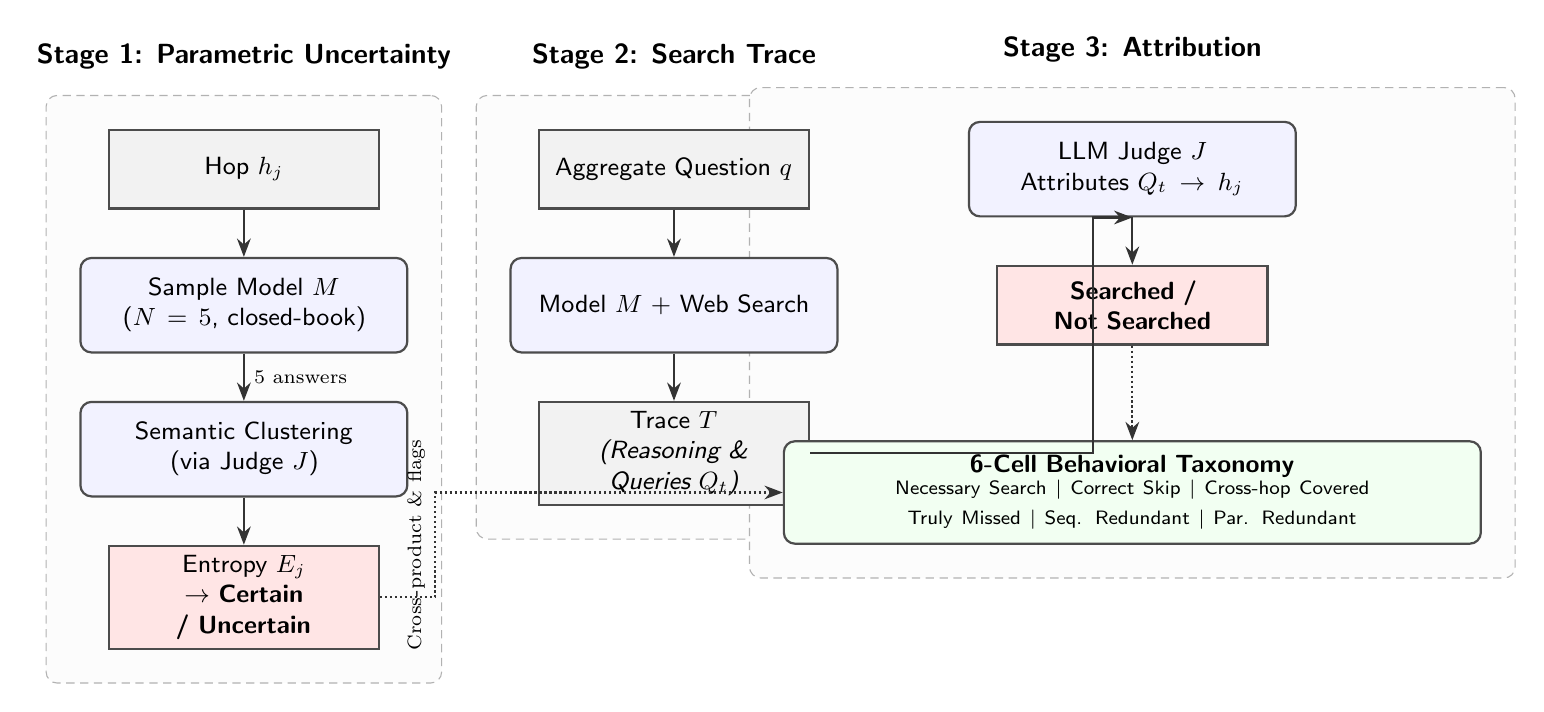
\begin{tikzpicture}[
    font=\sffamily\small,
    >=Stealth,
    % Define styles for the blocks
    block/.style={rectangle, draw=black!70, thick, rounded corners, fill=blue!5, text width=3.8cm, text centered, minimum height=1.2cm, inner sep=5pt},
    wideblock/.style={rectangle, draw=black!70, thick, rounded corners, fill=green!5, text width=8.5cm, text centered, minimum height=1.2cm, inner sep=5pt},
    doc/.style={rectangle, draw=black!70, thick, fill=gray!10, text width=3.2cm, text centered, minimum height=1cm},
    arrow/.style={thick, ->, draw=black!80},
    panel/.style={draw=black!30, densely dashed, rounded corners, inner sep=12pt, fill=gray!2}
]

% ==========================================
% Panel 1 (Left): Parametric Uncertainty
% ==========================================
\node[doc] (hop) {Hop $h_j$};
\node[block, below=0.6cm of hop] (sample) {Sample Model $M$\\($N=5$, closed-book)};
\node[block, below=0.6cm of sample] (cluster) {Semantic Clustering\\(via Judge $J$)};
\node[doc, below=0.6cm of cluster, fill=red!10] (certainty) {Entropy $E_j$\\ $\to$ \textbf{Certain / Uncertain}};

\begin{scope}[on background layer]
    \node[panel, fit=(hop) (sample) (cluster) (certainty)] (panel1) {};
    \node[above=0.2cm of panel1, font=\sffamily\bfseries] {Stage 1: Parametric Uncertainty};
\end{scope}

\draw[arrow] (hop) -- (sample);
\draw[arrow] (sample) -- node[right, font=\scriptsize] {5 answers} (cluster);
\draw[arrow] (cluster) -- (certainty);

% ==========================================
% Panel 2 (Middle): Search-Augmented Trace
% ==========================================
\node[doc, right=2cm of hop] (question) {Aggregate Question $q$};
\node[block, below=0.6cm of question] (searchrun) {Model $M$ + Web Search};
\node[doc, below=0.6cm of searchrun] (trace) {Trace $T$\\ \textit{(Reasoning \& Queries $Q_t$)}};

\begin{scope}[on background layer]
    \node[panel, fit=(question) (searchrun) (trace)] (panel2) {};
    \node[above=0.2cm of panel2, font=\sffamily\bfseries] {Stage 2: Search Trace};
\end{scope}

\draw[arrow] (question) -- (searchrun);
\draw[arrow] (searchrun) -- (trace);

% ==========================================
% Panel 3 (Right): Attribution & Taxonomy
% ==========================================
\node[block, right=2cm of question] (judge) {LLM Judge $J$\\ Attributes $Q_t \to h_j$};
\node[doc, below=0.6cm of judge, fill=red!10] (searched) {\textbf{Searched / Not Searched}};
\node[wideblock, below=1.2cm of searched] (taxonomy) {\textbf{6-Cell Behavioral Taxonomy}\\
{\scriptsize Necessary Search $\vert$ Correct Skip $\vert$ Cross-hop Covered \\ Truly Missed $\vert$ Seq. Redundant $\vert$ Par. Redundant}};

\begin{scope}[on background layer]
    \node[panel, fit=(judge) (searched) (taxonomy)] (panel3) {};
    \node[above=0.2cm of panel3, font=\sffamily\bfseries] {Stage 3: Attribution};
\end{scope}

% Route trace output to judge input
\draw[arrow] (trace.east) -| ([xshift=-0.5cm]judge.south) -- (judge.south);
\draw[arrow] (judge) -- (searched);

% Combine Certainty and Search behavior into Taxonomy
\draw[arrow, thick, densely dotted] (certainty.east) -- ++(0.7,0) |- (taxonomy.west) node[pos=0.25, above, sloped, font=\scriptsize] {Cross-product \& flags};
\draw[arrow, thick, densely dotted] (searched.south) -- (taxonomy.north);

\end{tikzpicture}%
}
\caption{\textbf{Protocol schematic.} \emph{Left:} For each hop $h_j$, the model is sampled $N{=}5$ times without search; semantic clustering yields the entropy $E_j$ and a \textsc{certain}/\textsc{uncertain} label. \emph{Middle:} The same model answers the aggregate question with web search enabled, producing a trace of interleaved reasoning and search calls. \emph{Right:} An LLM judge attributes each emitted query back to a specific hop; the cross-product of $\mathrm{certain}\times\mathrm{searched}$, refined with sequential-redundancy and cross-hop-coverage flags, yields the six-cell behavioural taxonomy used throughout the paper.}
\label{fig:protocol}
\end{figure*}

\paragraph{Stage 0 --- staleness filtering.}
MuSiQue contains time-sensitive questions (office-holders, populations) whose correct
action depends on external state rather than internal knowledge. An LLM judge flags
such items; we retain \textbf{600 non-stale multi-hop questions} as the evaluation set.

\paragraph{Stage 1 --- per-hop parametric uncertainty.}
We follow \citet{farquhar2024} and estimate uncertainty from $N{=}5$ closed-book
samples clustered into semantic equivalence classes, computing semantic entropy $E_j$
in bits. We use sampling-based rather than logit-based entropy because the Gemini API
does not expose per-token log-probabilities and because RLHF-sharpened token
distributions systematically under-estimate genuine ignorance
\citep{flare2023,farquhar2024}. A hop is \textbf{certain} iff $E_j = 0$ \emph{and} the
cluster matches the gold answer --- the conjunction guards against the confident-wrong
failure mode.

\paragraph{Stage 2 --- search-augmented run.}
The model receives the aggregate question and a Brave-Search-backed web tool; we
record the full trace and the final answer. Brave operates an independent web index
with no corporate product relationship to the three evaluated model vendors, reducing
provider-side confounds. We do not fine-tune any model.

\paragraph{Stage 3 --- query-to-hop attribution and trace flags.}
An LLM judge maps each emitted search query to a single hop using the hop questions and
the preceding reasoning as context; a secondary multi-hop pass validates this
simplification ($79$--$87\%$ of queries serve a single hop;
Appendix~\ref{app:operational:oneone}). Two trace-level flags enrich the binary
$\mathrm{searched}_{i,j}$: \texttt{seq\_redundant} marks hops whose search was
sequentially redundant within the trace, and \texttt{xhop\_cov} marks hops whose gold
answer was returned as a by-product of a query attributed to a different hop.

\paragraph{Six-cell behavioural taxonomy.}
Cross-tabulating these annotations partitions every per-hop decision into one of six
interpretable categories (Table~\ref{tab:cats}). Three are correct decisions; three
are search errors with distinct semantics. We will refer to these cells throughout the
paper.

\begin{table}[ht]
\centering
\small
\caption{The six search-calibration categories. The first three are correct
decisions; the remaining three are distinct error modes. ``Searched'' refers to whether
the LLM-judge attributed at least one search query to the hop. \texttt{seq\_red} =
sequentially redundant within the trace; \texttt{x-hop} = the gold-equivalent content was
returned by a query attributed to a different hop.}
\label{tab:cats}
\begin{tabular}{lcccc l}
\toprule
\textbf{Category} & \textbf{Certain?} & \textbf{Searched?} & \texttt{seq\_red} & \texttt{x-hop} & \textbf{Reading} \\
\midrule
Necessary search    & no  & yes & --   & --   & Correct: search was warranted \\
Correct skip        & yes & no  & --   & --   & Correct: model knew, did not waste a call \\
Cross-hop covered   & no  & no  & --   & yes  & Correct: hop recovered via another hop's query \\
\midrule
Truly missed        & no  & no  & --   & no   & Error: gap left open \\
Seq.\ redundant     & yes & yes & yes  & --   & Error: re-querying already-known content \\
Par.\ redundant     & yes & yes & no   & --   & Error: searching a hop the model knew \\
\bottomrule
\end{tabular}
\end{table}

\paragraph{Models.}
We evaluate \textbf{Gemini 3.1 Pro} (Google), \textbf{Qwen 3.5 122B} (Alibaba), and
\textbf{Nemotron Nano 30B} (NVIDIA) --- three vendors, three architectural families,
three independent training pipelines, spanning roughly one order of magnitude of
scale, all with native tool-use support. Behavioural patterns shared across all three
are therefore unlikely to reflect a common training artifact. Operational details
(serving, judge choice, search backend, paraphrase generation) are deferred wholesale
to Appendix~\ref{app:operational}.

% ============================================================================
\section{RQ1: Are Searches Aligned with Epistemic Uncertainty?}\label{sec:auroc}
% ============================================================================

\textbf{RQ1} asks whether a model searches a hop \emph{because} it is uncertain about
that hop --- the most direct test of whether the search policy is governed by the
model's own knowledge boundary. We test alignment with the AUROC of
$\text{entropy}\rightarrow\text{search}$: under an uncertainty-driven policy this
would approach $1.0$. We observe instead AUROC in the $0.56$--$0.62$ range across all
three models (Figure~\ref{fig:roc}).

\begin{figure}[ht]
\centering
\includegraphics[width=0.78\linewidth]{auroc_summary.pdf}
\caption{AUROC of semantic entropy as a predictor of the per-hop search decision, per
(model, dataset). The dashed line marks the random baseline (AUROC = 0.5). All six
combinations fall in the $0.53$--$0.62$ range; for Gemini under natural paraphrasing,
AUROC drops to $0.528$ --- effectively chance.}
\label{fig:roc}
\end{figure}

Two observations sharpen the finding. (1)~Even the best of the three, Nemotron, clears
AUROC 0.6 only modestly --- and pays for that small calibration advantage with the
highest \emph{Truly missed} rate (anticipated in \S\ref{sec:profile}), so what
alignment exists is purchased by coverage failure rather than by graded sensitivity.
(2)~The per-entropy search rate is roughly flat rather than monotone in $E_j$ for all
three models: search behaves as an approximately binary action with little graded
response to the magnitude of internal uncertainty (Appendix~\ref{app:binary}).

\paragraph{Verdict (RQ1).}
No --- search calls are barely aligned with the model's own epistemic uncertainty. The
latent uncertainty signal exists in the model and is measurable, but it is not the
dominant driver of when any of these three production-style LLMs decide to search.

\paragraph{Is this good behaviour?}
This is the most fundamental miscalibration we will see: a search policy that ignores
the model's own knowledge boundary cannot be good in either regime. But whether the
resulting errors land as costs (wasted retrieval) or as correctness failures
(uncovered gaps) depends on \emph{what specifically} gets mis-searched --- the
question we turn to next in \S\ref{sec:efficiency} and \S\ref{sec:profile}.

% ============================================================================
\section{RQ2: Are Search Calls Efficient?}\label{sec:efficiency}
% ============================================================================

If a model's searches are not driven by its own uncertainty (\S\ref{sec:auroc}), how
much of its query budget actually lands on the hops where it is needed?
\textbf{RQ2} asks this directly, formalised as the \emph{Search Budget Efficiency}
(SBE) --- the fraction of issued queries that target an uncertain hop, equivalently
one minus the wasted-search rate:
\[
  \mathrm{SBE} \;=\; \frac{N_{\text{queries on uncertain hops}}}{N_{\text{queries total}}}.
\]
SBE collapses both redundancy modes (parametric, sequential) into a single
``budget spent off-target'' rate. On the benchmark, Gemini scores
$\mathrm{SBE}=0.045$, Qwen $0.232$, and Nemotron $0.233$ (Figure~\ref{fig:sbe}): even
the best of the three spends roughly $77\%$ of its query budget off-target, and Gemini
spends $95\%$.

\begin{figure}[ht]
\centering
\includegraphics[width=0.78\linewidth]{fig3_search_budget_efficiency.pdf}
\caption{Search Budget Efficiency per model and per dataset. SBE is the fraction of
issued queries attributed to a hop with $E_j>0$ (an uncertain hop); the remainder is
wasted on parametrically- or sequentially-redundant searches. Higher is better.}
\label{fig:sbe}
\end{figure}

\paragraph{Verdict (RQ2).}
No --- between $\sim 77\%$ (Nemotron, Qwen) and $\sim 95\%$ (Gemini) of every model's
query budget is spent off-target relative to its own knowledge boundary.

\paragraph{Is this good behaviour?}
An SBE of $0.045$ is not a defensible operating point: the model is paying for an
order-of-magnitude more queries than it consumes information from. Even Nemotron's
$0.233$ means three-quarters of its budget is wasted. But the scalar number does not
tell us \emph{how} each model is inefficient --- whether the wasted spend is
double-checking facts already known (a cost) or leaving uncertain hops uncovered (a
correctness failure). That is RQ3.

% ============================================================================
\section{RQ3: Do Models Decompose Questions and Search Efficiently?}\label{sec:profile}
% ============================================================================

\textbf{RQ3} asks not just whether the search budget is efficient on aggregate (RQ2)
but \emph{how} each model's inefficiency is distributed across the six taxonomy cells
of Table~\ref{tab:cats} --- whether a model's failure is one of wasted searches or of
uncovered gaps. Decomposition itself is not in serious doubt: the LLM judge attributes
$79$--$87\%$ of queries to a single hop, confirming that all three models do
syntactically split the question into per-hop searches. What differs sharply is the
qualitative shape of the inefficiency.

Table~\ref{tab:profile} gives the full six-category breakdown per model on the
benchmark. The extended categories distinguish two flavours of redundancy (sequential
vs.\ parametric) and isolate the Cross-hop covered category, which a strict ``did the
model search this hop'' framing would otherwise mis-classify as a miss.

\begin{table}[ht]
\centering
\small
\caption{Search-calibration profile per model on MuSiQue (\% of 1800 hops). Left of
the rule: correct decisions. Right: distinct error modes.}
\label{tab:profile}
\begin{tabular}{l|ccc|ccc}
\toprule
 & \multicolumn{3}{c|}{\textbf{Correct}} & \multicolumn{3}{c}{\textbf{Errors}} \\
\textbf{Model} & \textbf{Necessary} & \textbf{Correct} & \textbf{Cross-hop} & \textbf{Truly} & \textbf{Seq.} & \textbf{Par.} \\
 & \textbf{search} & \textbf{skip} & \textbf{covered} & \textbf{missed} & \textbf{redundant} & \textbf{redundant} \\
\midrule
Gemini 3.1 Pro       & 44.7 & 15.6 & ~5.1 & ~5.1 & ~9.2 & \textbf{20.5} \\
Nemotron Nano 30B  & 43.3 & 15.4 & 10.2 & \textbf{24.3} & ~1.3 & ~5.4 \\
Qwen 3.5 122B      & \textbf{49.0} & 13.9 & ~7.7 & ~6.7 & ~2.8 & 19.8 \\
\bottomrule
\end{tabular}
\end{table}

\paragraph{Three model archetypes.} The category mix reveals qualitatively different
calibration failures:
\begin{itemize}[leftmargin=*,itemsep=2pt]
\item \textbf{Gemini} is a \emph{high-volume, redundancy-prone} searcher. Its dominant
error mode is \emph{Parametrically redundant} (20.5\%) plus \emph{Sequentially redundant}
(9.2\%) --- nearly 30\% of its hops are wasted searches on content it already has, either
in its parameters or in earlier turns of the trace. Coverage of uncertain hops, however,
is excellent: \emph{Truly missed} is only 5.1\%.
\item \textbf{Nemotron} is the inverse archetype --- a \emph{coverage-failing
under-searcher}. Redundancy of both kinds is small (1.3\% + 5.4\%), but
\emph{Truly missed} dominates at 24.3\%: nearly a quarter of all hops are uncertain and
the model never even attempts a query.
\item \textbf{Qwen} sits between the two. It searches more uncertain hops than the
other two (49.0\% \emph{Necessary search}) but pays for it with 19.8\% \emph{Par.\
redundant}, mirroring Gemini's redundancy pattern at slightly lower volume.
\end{itemize}
A Kruskal--Wallis test on the per-hop entropy distributions rejects the null of equal
distributions across the three models ($H=499.2$, $p<10^{-108}$), so the behavioural
differences are not driven by trivially different uncertainty inputs; full statistics
are in \texttt{statistical\_tests.csv}
(Appendix~\ref{app:operational:stats}).\footnote{A Mann--Whitney U test on the entropy
of \emph{searched} hops further shows Nemotron searches substantially more uncertain
hops on average than Gemini ($p<10^{-97}$), consistent with the two models' very
different positions on the redundancy/coverage axis.}

The three-way error decomposition is essential. Any binary collapse to ``correct
search-decision'' versus ``error'' would hide that Gemini and Nemotron fail in
opposite ways. Cross-hop coverage --- the case where an uncertain hop is recovered as
a by-product of another hop's query --- is non-negligible (5.1--10.2\%) for all three;
we count it as a correct outcome, since the hop's information need is in fact
satisfied, but it is invisible in a strict ``did the model search this hop'' framing
and would be misread as a miss without this annotation.

\paragraph{Verdict (RQ3).}
Yes on decomposition; no on efficiency. All three models split the question and
dispatch hop-level queries, but the resulting per-hop search profile is dominated by
distinct error modes: redundancy for Gemini and Qwen, missed coverage for Nemotron.

\paragraph{Is this good behaviour?}
The three archetypes are not equally bad. Gemini's redundancy spend wastes latency
and dollars but rarely loses correctness; Nemotron's coverage gaps directly cost
answer correctness; Qwen sits between the two. Which is preferable depends on whether
the deployment context tolerates latency or hallucination --- a tension we return to
in \S\ref{sec:discussion}.

% ============================================================================
\section{RQ4: Do Models Behave Differently on User-Style Questions?}\label{sec:paraphrase}
% ============================================================================

\textbf{RQ4} asks whether the behavioural profile we have just measured transfers to
questions phrased the way a real user would phrase them. MuSiQue exposes the hop chain
syntactically (``What administrative territorial entity includes the place where X was
educated?''). A genuine user with the same information need would phrase the question
differently (``I'm curious about X's background --- what region of the country did he
study in?''). The information need is identical (same gold answer, same hop chain),
but the surface form differs: no nested relative clauses, no exposed bridge entities,
often a request for a short narrative rather than a single fact. If the search-decision
policy were governed by the model's internal uncertainty about facts, behaviour should
be approximately invariant to this surface change. We test this directly by rewriting
each of the 600 MuSiQue questions into a natural, goal-oriented paraphrase under three
verifiable constraints (no bridge entities named, no exposed relative-clause hop
structure, phrasing that invites 2--4 explanatory sentences;
Appendix~\ref{app:operational:paraphrase}) and re-running only Stages~2--3.

\paragraph{Observation 1 --- Search volume collapses.}
All three models cut search volume substantially (Table~\ref{tab:volume}): Qwen by
$4.2\times$, Gemini by $3.1\times$, Nemotron by $1.8\times$. The information need is
identical; only the phrasing changed.

\begin{table}[ht]
\centering
\small
\caption{Search volume per question, benchmark vs.\ natural paraphrase (paired across
600 items). Wilcoxon signed-rank test, two-sided.}
\label{tab:volume}
\begin{tabular}{lcccc}
\toprule
\textbf{Model} & \textbf{Benchmark (mean)} & \textbf{Natural (mean)} & \textbf{Ratio} & \textbf{Wilcoxon $p$} \\
\midrule
Gemini 3.1 Pro       & 15.20 & 4.93 & $3.1\times$ & $3.0\!\times\!10^{-73}$ \\
Nemotron Nano 30B  &  5.74 & 3.13 & $1.8\times$ & $2.4\!\times\!10^{-21}$ \\
Qwen 3.5 122B      &  5.60 & 1.33 & $4.2\times$ & $6.4\!\times\!10^{-88}$ \\
\bottomrule
\end{tabular}
\end{table}

\paragraph{Observation 2 --- Calibration collapses: the wrong cells grow.}
Reduced search would be unsurprising if the model's calibration \emph{survived}: a leaner
search budget could still be allocated to uncertain hops. It does not.
Table~\ref{tab:shift} shows the six-category shift from benchmark to natural paraphrase
for each model. The pattern is uniform across models: \emph{Necessary search}
collapses by 11--27 percentage points, and the lost mass moves predominantly into
\emph{Truly missed} (uncertain hop the model fails to search at all). \emph{Par.\
redundant} also drops --- which would be a positive in isolation --- but the trade-off is
unfavourable: the model loses correct searches faster than it loses wasted ones.

\begin{table}[ht]
\centering
\footnotesize
\caption{Six-category profile shift under natural paraphrasing
($\Delta=\text{Natural}-\text{Benchmark}$, in percentage points of 1800 hops). All three
models lose \emph{Necessary search} and gain \emph{Truly missed}.}
\label{tab:shift}
\setlength{\tabcolsep}{4pt}
\begin{tabular}{l|ccc|ccc}
\toprule
 & \multicolumn{3}{c|}{\textbf{Correct}} & \multicolumn{3}{c}{\textbf{Errors}} \\
\textbf{Model} & $\Delta$Nec.\ srch. & $\Delta$Corr.\ skip & $\Delta$X-hop cov. & $\Delta$Truly miss. & $\Delta$Seq.\ red. & $\Delta$Par.\ red. \\
\midrule
Gemini 3.1 Pro       & $-19.4$ & $+14.3$ & $+2.0$ & $\mathbf{+17.3}$ & $-6.1$ & $-8.2$ \\
Nemotron Nano 30B  & $-10.5$ & $+3.4$  & $+1.4$ & $\mathbf{+9.2}$  & $-0.7$ & $-2.7$ \\
Qwen 3.5 122B      & $-27.4$ & $+15.5$ & $-0.3$ & $\mathbf{+27.7}$ & $-2.4$ & $-13.1$ \\
\bottomrule
\end{tabular}
\end{table}

\paragraph{Observation 3 --- The calibration gap persists or widens.}
Under natural paraphrasing the AUROC of $\text{entropy}\rightarrow\text{search}$ drops
marginally for Gemini ($0.557\to 0.528$) and is essentially unchanged for the two open
models. RQ1's finding --- that entropy is a weak predictor of search --- \emph{persists
and degrades for the highest-volume searcher}. Surface form, not internal uncertainty,
governs the policy.

\paragraph{The headline picture.}
Figure~\ref{fig:quadrant_taxonomy} compresses the shift into a single chart: the
four-cell (E\,/\,PR\,/\,M\,/\,CP) collapse of the six-category profile per model and
per dataset, with each (model, dataset) bar summing to 100\% of its 1800 hops. Reading
left-to-right, the first three bars are the three models on benchmark MuSiQue and the
next three are the same models on the natural paraphrase. Across all three models the
red \emph{Missed} segment expands sharply, the green \emph{Effective} segment
contracts, and the orange \emph{Parametrically Redundant} segment also shrinks --- but
the shrinkage of PR is not a saving, because the same models lose Effective search
faster than they lose wasted search.

\begin{figure}[ht]
\centering
\includegraphics[width=0.95\linewidth]{fig1_quadrant_taxonomy.pdf}
\caption{\textbf{Headline figure for RQ4.} Four-cell taxonomy collapse of the
six-category profile (E~=~Effective / Necessary search, CP~=~Correct skip,
PR~=~Parametrically Redundant, M~=~Missed) per model and per dataset. Each bar sums to
100\% of that (model, dataset)'s 1800 hops. The natural-paraphrase bars show a uniform
expansion of red (Missed) and contraction of green (Effective).}
\label{fig:quadrant_taxonomy}
\end{figure}

The per-model extended profile of Figure~\ref{fig:cal_one} (Gemini; remaining two
models in Appendix~\ref{app:other_cal}) confirms the cell-level direction of the shift.
A complementary appendix probe (Appendix~\ref{app:cascade}) shows that the growth in
\emph{Truly missed} is dominated by \emph{genuine} misses rather than by downstream
cascade failures from a wrong earlier hop, so the shift is not an artifact of
upstream errors.

\begin{figure}[ht]
\centering

\includegraphics[width=0.92\linewidth]{search_calibration_extended_gemini_3_pro_preview.pdf}
\caption{Extended search-calibration profile for Gemini 3.1 Pro. Solid bars: benchmark
MuSiQue; hatched bars: natural paraphrase. Left of the dashed line are correct
decisions; right are the three error categories. The benchmark$\to$natural shift moves
mass from Necessary search into Truly missed (and from Par.\ redundant into Correct
skip), the calibration regression Table~\ref{tab:shift} quantifies. The other two
models are in Figure~\ref{fig:cal_others}.}
\label{fig:cal_one}
\end{figure}

\paragraph{Verdict (RQ4).}
Yes --- behaviour changes sharply under a cosmetic paraphrase that preserves the
information need, and the change is not benign. All three models search less, the
remaining searches are re-allocated \emph{away} from uncertain hops, and the dominant
new error cell is \emph{Truly missed}: an uncertain hop the model never queries the
web for. The model's internal knowledge boundary has not moved; only the surface form
of the question has.

\paragraph{Is this good behaviour?}
No. The shift is not benign: under benchmark framing the error budget concentrates in
\emph{Parametrically Redundant} (PR --- wasted but recoverable; the user pays in
latency); under natural framing it concentrates in \emph{Truly missed} (M ---
an answer-correctness failure). The natural regime trades cost-flavoured errors for
correctness-flavoured errors --- a strictly worse exchange from the user's
perspective. This re-allocation is the load-bearing piece of the Discussion.

% ============================================================================
\section{Discussion}\label{sec:discussion}
% ============================================================================

\paragraph{Synthesis: which behaviour is better, and in what cases?}
The four results sections each closed with a reflection on whether the observed
behaviour is good; here we pull those reflections together. The benchmark regime is
the more searched-on, more redundancy-prone of the two: every model's error budget
under benchmark framing concentrates in \emph{Parametrically} and \emph{Sequentially
Redundant} searches --- queries the model did not need to issue, paid for in latency
and dollars but rarely costing correctness. Under natural framing the error budget
migrates into \emph{Truly missed} (Table~\ref{tab:shift}: $+17$, $+9$, $+28$
percentage points for Gemini, Nemotron, Qwen), a strictly worse currency: an uncertain
hop never queried and never covered, so the answer either hallucinates or omits the
information need. Across deployment contexts the choice is not symmetric. In
latency-sensitive applications where wrong answers can be tolerated downstream,
the benchmark regime's redundancy is the smaller harm; in correctness-sensitive
applications where a confident wrong answer is the worst possible failure, even the
benchmark regime is not safe and the natural regime is unacceptable. The same
re-allocation argument applies across models: Gemini's redundancy is a cost,
Nemotron's missed coverage is a failure, Qwen's mix is the intermediate trade-off ---
and the cost-vs-failure axis, not raw search volume, is the right ordering principle.

\paragraph{Why framing flips the policy --- the commitment-locus mechanism.}
A behavioural probe localises \emph{when} in the trace the regression happens
(full results in Appendix~\ref{app:commit}). For every (example, hop, variant) pair an
LLM judge identifies the first turn at which the agent commits to a per-hop answer.
The decisive cell is \texttt{commit\_no\_search}: the agent settled on an answer for
that hop and no search was ever attributed to it. Under benchmark framing, Gemini
exhibits this pattern on 22.6\% of hops; under natural framing the rate jumps to
51.9\%. Qwen rises 18.0\% $\to$ 38.5\%. The model is not ``forgetting'' to search ---
it is \emph{deciding} the answer earlier, before any search query is issued. This is a
behavioral analogue of the ``context leads, parametric memory follows'' effect of
\citet{tao2024context}: here the \emph{search-decision} policy, not the answer,
conditions on the prompt's surface register, consistent with the
mechanistic account of \citet{knowingdoing2026} in which a model's tool-recognition
and tool-execution representations become nearly orthogonal under conversational
framing.

\paragraph{Implications for tool-use training.}
The standard RAG / tool-use training paradigm --- Toolformer-style supervised insertion
\citep{toolformer2023}, Self-RAG critique tokens \citep{selfrag2024}, distillation from
agentic trajectories \citep{rare2025} --- does not explicitly tie the decision to
search to the model's own uncertainty about the sub-step. Methods that close this loop
--- e.g.\ S-GRPO \citep{sgrpo2025}, which rewards search only when the model's belief
warrants it --- exist but are not yet the dominant paradigm. Our protocol offers a
diagnostic complement to these training-time fixes: it measures, on a held-out set,
whether a given training method actually closes the calibration gap on both benchmark
and user-style framings.

\paragraph{Limitations.}
(i)~Per-hop attribution uses an LLM judge; the one-query--one-hop simplification is
validated in Appendix~\ref{app:operational:oneone}.
(ii)~Sampling-based entropy at $N{=}5$ gives a coarse seven-value uncertainty
resolution; we do not probe logits because the Gemini API does not expose them.
Richer probes \citep{evidential2026,sep2024} may sharpen the signal.
(iii)~MuSiQue is the only multi-hop benchmark we evaluate, because it is the only one
that provides the gold hop decomposition our Stage~1 protocol needs; generalisation to
other multi-hop datasets is left to future work.
(iv)~We do not vary the search backend; results may differ with stronger retrieval.
(v)~Only one paraphrase per question is evaluated; the generalization gap may be
larger across the full natural-language manifold.

% ============================================================================
\section{Conclusion}
% ============================================================================

Info-seeking queries put parametric memory and live web search in continuous tension.
Existing benchmarks tell us whether RAG helps on aggregate; they do not tell us
whether a model knows \emph{when} to defer to its parameters and when to reach for the
web. The protocol introduced here asks this question directly, grounded in per-hop
semantic entropy paired with per-hop search attribution. Applied to three
production-style LLMs (Gemini 3.1 Pro, Qwen 3.5 122B, Nemotron Nano 30B), it produces
the following one-line verdicts:
\begin{itemize}[leftmargin=*,itemsep=2pt]
\item \textbf{RQ1.} No --- search calls are barely aligned with internal uncertainty;
the AUROC of $\text{entropy}\rightarrow\text{search}$ sits in 0.53--0.62, barely
above chance, and search is approximately binary in internal uncertainty.
\item \textbf{RQ2.} No --- Search Budget Efficiency ranges from 0.045 (Gemini) to
0.233 (Nemotron), so between 77\% and 95\% of every model's query budget is spent
off-target.
\item \textbf{RQ3.} Yes on decomposition; no on efficiency. All three models split
the question (79--87\% one-to-one query-to-hop attribution) but exhibit qualitatively
different inefficiency profiles: redundancy-prone (Gemini), coverage-failing
(Nemotron), or in between (Qwen).
\item \textbf{RQ4.} Yes --- a cosmetic, meaning-preserving paraphrase causes every
model to behave very differently. Search volume drops $1.8$--$4.2\times$ and the
remaining searches are re-allocated \emph{away} from the same uncertain hops the
model identified on the benchmark, with \emph{Truly missed} becoming the dominant
error cell.
\end{itemize}
Together these constitute a hidden generalization gap in the
parametric$\leftrightarrow$search interplay of contemporary info-seeking LLMs. As both
axes of model capability --- parametric knowledge and agentic tool use --- continue to
advance, the protocol introduced here is a starting point for measuring, and
ultimately closing, that gap.

% ============================================================================
% References — replace with \bibliography{refs} once a .bib file is finalized.
% ============================================================================
\begin{thebibliography}{99}\setlength{\itemsep}{1pt}

\bibitem[Asai et al.(2024)]{selfrag2024}
A. Asai, Z. Wu, Y. Wang, A. Sil, and H. Hajishirzi.
Self-{RAG}: Learning to retrieve, generate, and critique through self-reflection.
\emph{ICLR}, 2024.

\bibitem[Cheng et al.(2024a)]{cheng2024interplay}
S. Cheng, L. Pan, X. Yin, X. Wang, and W. Y. Wang.
Understanding the interplay between parametric and contextual knowledge for large language models.
\emph{arXiv:2410.08414}, 2024.

\bibitem[Farahani and Johansson(2024)]{farahani2024deciphering}
M. Farahani and R. Johansson.
Deciphering the interplay of parametric and non-parametric memory in retrieval-augmented language models.
\emph{EMNLP}, 2024.

\bibitem[Farquhar et al.(2024)]{farquhar2024}
S. Farquhar, J. Kossen, L. Kuhn, and Y. Gal.
Detecting hallucinations in large language models using semantic entropy.
\emph{Nature}, 630(8017):625--630, 2024.

\bibitem[Huang and Huang(2024)]{huang2024rag}
Y. Huang and J. X. Huang.
A survey on retrieval-augmented text generation for large language models.
\emph{ACM Computing Surveys}, 2024.

\bibitem[Kim et al.(2025)]{kim2025reliability}
Y. Kim et al.
Reliability across parametric and external knowledge: Understanding knowledge handling in {LLMs}.
\emph{arXiv:2502.13648}, 2025.

\bibitem[Kunitomo-Jacquin et al.(2026)]{evidential2026}
L. Kunitomo-Jacquin et al.
Evidential semantic entropy for {LLM} uncertainty quantification.
\emph{EACL}, 2026.

\bibitem[Lee and Hockenmaier(2025)]{lee2025reasoningtraces}
J. Lee and J. Hockenmaier.
Evaluating step-by-step reasoning traces: A survey.
\emph{arXiv:2502.12289}, 2025.

\bibitem[Li et al.(2024)]{li2024patching}
Z. Li et al.
Understanding and patching compositional reasoning in {LLMs}.
\emph{Findings of ACL}, 2024.

\bibitem[Min et al.(2023)]{factscore2023}
S. Min et al.
{FActScore}: Fine-grained atomic evaluation of factual precision in long-form text generation.
\emph{EMNLP}, 2023.

\bibitem[Ning et al.(2024)]{wtu2024}
K. Ning et al.
{WTU-Eval}: A whether-or-not tool usage evaluation benchmark for large language models.
\emph{arXiv:2407.12823}, 2024.

\bibitem[Schick et al.(2023)]{toolformer2023}
T. Schick et al.
Toolformer: Language models can teach themselves to use tools.
\emph{NeurIPS}, 2023.

\bibitem[Tao et al.(2024)]{tao2024context}
Y. Tao et al.
When context leads but parametric memory follows in large language models.
\emph{EMNLP}, 2024.

\bibitem[Trivedi et al.(2022)]{musique}
H. Trivedi, N. Balasubramanian, T. Khot, and A. Sabharwal.
{MuSiQue}: Multihop questions via single-hop question composition.
\emph{TACL}, 10:539--554, 2022.

\bibitem[Wadhwa et al.(2026)]{wadhwa2026rags}
H. Wadhwa et al.
From {RAGs} to rich parameters: Probing how language models utilize external knowledge over parametric information for factual queries.
\emph{WSDM}, 2026.

\bibitem[Wang et al.(2025b)]{rare2025}
Z. Wang, A. Mao, H. Wu, T. Bui, J. Wang, Y. Tang, Y. Li, Y. Zhuang, J. Kang, S. C. H. Hoi, and W. Wang.
{RARE}: Retrieval-augmented reasoning modeling.
\emph{arXiv:2503.23513}, 2025.

\bibitem[Wu et al.(2024a)]{wu2024clasheval}
K. Wu, E. Wu, and J. Zou.
{ClashEval}: Quantifying the tug-of-war between an {LLM}'s internal prior and external evidence.
\emph{NeurIPS}, 2024.

\bibitem[Wu et al.(2024b)]{wu2024mrke}
J. Wu et al.
{MRKE}: The multi-hop reasoning evaluation of {LLMs} by knowledge edition.
\emph{arXiv:2402.11924}, 2024.

\bibitem[Yang et al.(2024)]{yang2024latent}
S. Yang et al.
Do large language models latently perform multi-hop reasoning?
\emph{ACL}, 2024.

\bibitem[Zhang et al.(2024)]{zhang2024fusion}
H. Zhang et al.
Evaluating the external and parametric knowledge fusion of large language models.
\emph{arXiv:2405.19010}, 2024.

\bibitem[Jiang et al.(2023)]{flare2023}
Z. Jiang, F. Xu, L. Gao, Z. Sun, Q. Liu, J. Dwivedi-Yu, Y. Yang, J. Callan, and G. Neubig.
Active retrieval augmented generation.
\emph{EMNLP}, 2023.

\bibitem[Guan et al.(2025)]{deeprag2025}
X. Guan, J. Zeng, F. Meng, C. Xin, Y. Lu, H. Lin, X. Han, L. Sun, and J. Zhou.
{DeepRAG}: Thinking to retrieve step by step for large language models.
\emph{arXiv:2502.01142}, 2025.

\bibitem[Wu et al.(2025a)]{hiprag2025}
P. Wu, M. Zhang, Z. Sheng, S. Wang, X. Du, and Z. Chen.
{HiPRAG}: Hierarchical process rewards for efficient agentic retrieval augmented generation.
\emph{arXiv:2510.07794}, 2025.

\bibitem[Guo et al.(2026)]{realmretrieve2026}
D. Guo, J. Wu, and S. M. Yiu.
When to retrieve during reasoning: Adaptive retrieval for large reasoning models.
\emph{arXiv:2604.26649}, 2026.

\bibitem[Qian et al.(2025)]{smarter2025}
C. Qian, E. C. Acikgoz, H. Wang, X. Chen, A. Sil, D. Hakkani-T\"ur, G. Tur, and H. Ji.
{SMART}: Self-aware agent for tool overuse mitigation.
\emph{Findings of ACL}, 2025.

\bibitem[Wu et al.(2025b)]{betaGRPO2025}
P. Wu, M. Zhang, X. Zhang, X. Du, and Z. Chen.
Search wisely: Mitigating sub-optimal agentic searches by reducing uncertainty.
\emph{EMNLP}, 2025.

\bibitem[Jang et al.(2026)]{howask2026}
Y. Jang et al.
How you ask matters! {A}daptive {RAG} robustness to query variations.
\emph{arXiv:2604.10745}, 2026.

\bibitem[Cheng et al.(2026)]{knowingdoing2026}
Y. Cheng, C. Fan, M. JafariRaviz, K. Rezaei, and S. Feizi.
Model-adaptive tool necessity reveals the knowing-doing gap in {LLM} tool use.
\emph{arXiv:2605.14038}, 2026.

\bibitem[Rabinovich et al.(2025)]{rabinovich2025agentic}
M. Rabinovich, A. Anaby-Tavor, et al.
On the robustness of agentic function calling.
\emph{TrustNLP workshop, NAACL}, 2025.

\bibitem[Wang et al.(2025c)]{towardtheory2025}
H. Wang, C. Qian, Y. Liu, J. Liu, Z. Du, M. He, B. Hu, K.-F. Wong, and H. Ji.
Position: Agent should invoke external tools only when epistemically necessary.
\emph{ICML Position Track}, 2025.

\bibitem[Wang et al.(2026)]{targ2026}
Y. Wang, L. Wei, and H. Ling.
Retrieval as a decision: Training-free adaptive gating for efficient {RAG}.
\emph{TMLR}, 2026.

\bibitem[Zubkova et al.(2025)]{sugar2025}
H. Zubkova, J.-H. Park, and S.-W. Lee.
{SUGAR}: Leveraging contextual confidence for smarter retrieval.
\emph{ICASSP}, 2025.

\bibitem[Yao et al.(2025)]{seakr2025}
Z. Yao et al.
{SeaKR}: Self-aware knowledge retrieval for adaptive retrieval augmented generation.
\emph{ACL}, 2025.

\bibitem[SEARAG(2025)]{searag2025}
{SEARAG}: Semantic entropy-guided adaptive retrieval for multi-hop question answering.
\emph{OpenReview submission} \url{https://openreview.net/forum?id=suKWySDjil}, 2025.

\bibitem[Kossen et al.(2024)]{sep2024}
J. Kossen et al.
Semantic entropy probes: Robust and cheap hallucination detection in {LLMs}.
\emph{arXiv:2406.15927}, 2024.

\bibitem[He et al.(2024)]{mintqa2024}
He, Hu et al.
{MINTQA}: A multi-hop question answering benchmark for evaluating {LLMs} on new and tail knowledge.
\emph{arXiv:2412.17032}, 2024.

\bibitem[Han et al.(2025)]{han2025judgeverdict}
H. Han et al.
Judge's verdict: A comprehensive analysis of {LLM} judge capability through human agreement.
\emph{arXiv:2510.09738}, 2025.

\bibitem[Wang et al.(2025a)]{adacad2025}
H. Wang, A. Prasad, E. Stengel-Eskin, and M. Bansal.
{AdaCAD}: Adaptively decoding to balance conflicts between contextual and parametric knowledge.
\emph{NAACL}, 2025.

\bibitem[Khandelwal et al.(2025)]{cocoa2025}
Khandelwal et al.
{CoCoA}: Confidence- and context-aware adaptive decoding for resolving knowledge conflicts in {LLMs}.
\emph{EMNLP}, 2025.

\bibitem[Huo et al.(2025)]{microact2025}
Huo et al.
Micro-{A}ct: Mitigate knowledge conflict in question answering via actionable self-reasoning.
\emph{ACL}, 2025.

\bibitem[Min et al.(2025)]{qucoraq2024}
D. Min, N. Zhang, Y. Yao, X. Wang, J. Du, S. Deng, H. Chen, and J. Pujara.
{QuCo-RAG}: Quantifying uncertainty from the pre-training corpus for dynamic retrieval-augmented generation.
\emph{arXiv:2512.19134}, 2025.

\bibitem[Cheng et al.(2024b)]{uar2024}
Q. Cheng, X. Li, S. Li, Q. Zhu, Z. Yin, Y. Shao, L. Li, T. Sun, H. Yan, and X. Qiu.
Unified active retrieval for retrieval augmented generation.
\emph{Findings of EMNLP}, 2024.

\bibitem[Li et al.(2025)]{r3rag2025}
Y. Li, Q. Luo, X. Li, B. Li, Q. Cheng, Y. Zheng, Z. Yin, P. Wang, B. Yu, and X. Qiu.
{R3-RAG}: Learning step-by-step reasoning and retrieval for {LLMs} via reinforcement learning.
\emph{Findings of EMNLP}, 2025.

\bibitem[Suri et al.(2025)]{sgrpo2025}
M. Suri, P. Mathur, N. Lipka, F. Dernoncourt, R. A. Rossi, and D. Manocha.
Structured uncertainty guided clarification for {LLM} agents.
\emph{arXiv:2511.08798}, 2025.

\end{thebibliography}

% ============================================================================
\appendix
% ============================================================================

\section{Extended Search-Calibration Plots for Nemotron and Qwen}\label{app:other_cal}

Per-model extended-calibration plots for the two models not shown in \S\ref{sec:profile}.
The bars use the same colour code as Figure~\ref{fig:cal_one}: green / blue / purple on
the left of the dashed line are correct decisions; orange / yellow / red on the right are
the three distinct error categories.

\begin{figure}[ht]
\centering
\begin{subfigure}{0.85\linewidth}
  
\includegraphics[width=\linewidth]{search_calibration_extended_nemotron_3_nano_30b.pdf}
  \caption{Nemotron Nano 30B --- coverage-failing under-searcher: \emph{Truly missed}
  dominates (24.3\% on the benchmark, 33.5\% on natural), while both redundancy
  categories stay small.}
\end{subfigure}\\[6pt]
\begin{subfigure}{0.85\linewidth}
  
\includegraphics[width=\linewidth]{search_calibration_extended_qwen3_5_122b.pdf}
  \caption{Qwen 3.5 122B --- the most aggressive volume drop under natural paraphrasing
  (search rate $4.2\times$ lower), with \emph{Truly missed} expanding from 6.7\% to
  34.4\%.}
\end{subfigure}
\caption{Extended search-calibration profiles for the remaining two models.}
\label{fig:cal_others}
\end{figure}

\section{Binary Search Behavior across Entropy Levels}\label{app:binary}

A direct calibration view plots the search rate $P(\text{searched}\mid H=h)$ as a function
of the discrete entropy level $h$ produced by $N=5$ closed-book sampling. Under
well-calibrated behavior, this curve would rise monotonically from $H{=}0$ (the model
should rarely search; it knows the answer) to $H{=}2.32$ (the model should almost always
search; it has near-uniform disagreement across samples). What we observe instead
(Figure~\ref{fig:per_h_rate}) is a roughly flat curve for all three models: the search
rate at $H{=}0$ is only a little below the rate at the highest entropy levels, and the
intermediate levels are noisy. A $\chi^2$ test of uniformity across entropy levels does
reject the null for every model ($p<10^{-4}$), so a small signal is statistically
present --- but the practical shape is binary: the model either searches at a
roughly-constant rate or it doesn't, with little graded sensitivity to how uncertain it
is. This is the per-entropy view of the near-chance AUROC reported in \S\ref{sec:auroc}.

\begin{figure}[ht]
\centering
\includegraphics[width=\linewidth,height=0.42\textheight,keepaspectratio]{searches_per_entropy_level.pdf}
\caption{Search rate $P(\text{searched}\mid H=h)$ per entropy level, per model, on
MuSiQue (left panel) and MuSiQue (Natural) (right panel). A well-calibrated policy
would rise monotonically from $H{=}0$ to $H{=}2.32$. Observed curves are roughly flat
on both datasets: behavior is approximately binary rather than graded with internal
uncertainty. Shaded band = 95\% Wilson CI.}
\label{fig:per_h_rate}
\end{figure}

% ----------------------------------------------------------------------
\section{Commitment-Locus Probe}\label{app:commit}

\paragraph{Motivation.}
If natural framing causes models to skip searches they would otherwise have issued,
\emph{when} does the skip happen? One hypothesis is that the casual register of the
paraphrased question invites a quick narrative answer, leading the model to commit to a
per-hop answer early --- before any search query is issued for that hop. The
\emph{commitment-locus probe} tests this directly.

\paragraph{Probe.}
For every (example, hop, variant) appearing in both the benchmark trace and the natural
trace of the same model, an LLM judge (\texttt{gpt-oss:120b}) identifies the first turn
at which the agent commits to a specific per-hop answer (asserts ``X is Y'' or treats Y
as established and uses it downstream). Combined with the first turn at which a search
query is attributed to that hop, this yields \texttt{committed\_before\_search} per
(hop, variant). The decisive cell is \texttt{commit\_no\_search}: the agent committed to
an answer for that hop and no search was ever attributed to it.

\paragraph{Result.}
Table~\ref{tab:commitment} reports the headline rates; Figure~\ref{fig:commit_early}
visualizes them. Across all three models, the rate of pre-search commitment rises
substantially under natural framing. For Gemini, commitment-without-search jumps from
22.6\% of hops on the benchmark to 51.9\% on the natural rewrite. For Qwen the rise is
18.0\% $\to$ 38.5\%. Nemotron, which already searched the least on the benchmark, shows
a smaller absolute increase.

\begin{table}[ht]
\centering
\small
\caption{Commitment-locus rates per (model, variant). \texttt{commit\_before\_search}:
agent committed before any search query attributed to the hop.
\texttt{commit\_no\_search}: agent committed and no search ever attributed.}
\label{tab:commitment}
\begin{tabular}{llccc}
\toprule
\textbf{Model} & \textbf{Variant} & \textbf{Committed at all} & \textbf{Before search} & \textbf{No search at all} \\
\midrule
\multirow{2}{*}{Gemini 3.1 Pro}      & Benchmark & 78.5\% & 34.7\% & 22.6\% \\
                                   & Natural   & 56.1\% & \textbf{52.2\%} & \textbf{51.9\%} \\
\multirow{2}{*}{Nemotron Nano}     & Benchmark & 52.2\% & 22.1\% & 21.5\% \\
                                   & Natural   & 54.0\% & 28.1\% & 27.8\% \\
\multirow{2}{*}{Qwen 3.5 122B}     & Benchmark & 75.9\% & 19.6\% & 18.0\% \\
                                   & Natural   & 61.7\% & \textbf{38.9\%} & \textbf{38.5\%} \\
\bottomrule
\end{tabular}
\end{table}

\begin{figure}[ht]
\centering
\includegraphics[width=0.78\linewidth]{fig1_early_commit_rate.png}
\caption{Pre-search commitment rate per (model, variant). Natural framing materially
shifts the locus of the per-hop answer to \emph{before} any search query is issued.}
\label{fig:commit_early}
\end{figure}

\begin{figure}[ht]
\centering
\includegraphics[width=0.78\linewidth]{fig2_fate_breakdown.png}
\caption{Commitment-fate breakdown per (model, variant). The growth of the orange
``committed without searching'' band under natural framing is the per-model picture of
the generalization gap localized to a single behavioral mechanism.}
\label{fig:commit_fate}
\end{figure}

\paragraph{Interpretation.}
The shift in commitment locus is a mechanistic explanation for the \emph{Truly missed}
growth reported in \S\ref{sec:paraphrase}: under natural framing the model is not simply
``forgetting'' to search --- it is \emph{deciding} the answer earlier, often before any
search would be triggered. This is consistent with the ``context leads, parametric memory
follows'' phenomenon of \citet{tao2024context}, re-cast at the level of the
\emph{search-decision} policy rather than the answer-generation policy.

% ----------------------------------------------------------------------
\section{Missed-Hop Confounder Analysis}\label{app:cascade}

\paragraph{Motivation.}
\emph{Truly missed} is the cell that grows the most under natural paraphrasing
(Table~\ref{tab:shift}). A potential confound is that some of these misses are not the
model's failure to act on its own uncertainty but downstream casualties of an earlier
mistake: if hop $k$ resolves to a wrong entity, the model has nothing to anchor a query
for hop $k{+}1$. We separate the two.

\paragraph{Decomposition.}
For each hop in the \emph{Truly missed} cell, we classify:
\begin{itemize}[leftmargin=*,itemsep=2pt]
\item \textbf{genuine\_missed}: $\text{hop\_index}=0$, or every prior hop's parametric
runs were all correct. The model could have searched and chose not to.
\item \textbf{cascade\_possible}: $\text{hop\_index}>0$ and at least one prior hop had
parametric accuracy $<1.0$. The model may have been ``starved'' of the anchor entity.
\end{itemize}
The auxiliary classifier \texttt{missed\_search\_answer\_found\_cross\_hop} ---
used to verify that a missed gold answer was \emph{not} present in any other hop's
search results before counting the hop as missed --- is the same
\texttt{gpt-oss:120b} judge used for query-to-hop attribution
(Appendix~\ref{app:operational:judges}).

\paragraph{Result.}
Table~\ref{tab:cascade} and Figure~\ref{fig:cascade_bar} show that the growth in
\emph{Truly missed} under natural paraphrasing is dominated by the
\emph{genuine\_missed} component for all three models. Genuine misses roughly triple for
Gemini (84~$\to$~277) and triple-plus for Qwen (105~$\to$~369); Nemotron rises by 42\%
(240~$\to$~342). This rules out the trivial explanation that the natural-paraphrase
generalization gap is a downstream casualty of upstream error.

\begin{table}[ht]
\centering
\small
\caption{\emph{Truly missed} decomposition: genuine misses vs.\ cascade-possible misses,
per (model, variant). Counts are of hops in the missed cell.}
\label{tab:cascade}
\begin{tabular}{llcc}
\toprule
\textbf{Model} & \textbf{Variant} & \textbf{Cascade possible} & \textbf{Genuine missed} \\
\midrule
\multirow{2}{*}{Gemini 3.1 Pro}     & Benchmark &  98 &  84 \\
                                  & Natural   & 254 & \textbf{277} \\
\multirow{2}{*}{Nemotron Nano}    & Benchmark & 382 & 240 \\
                                  & Natural   & 470 & \textbf{342} \\
\multirow{2}{*}{Qwen 3.5 122B}    & Benchmark & 155 & 105 \\
                                  & Natural   & 385 & \textbf{369} \\
\bottomrule
\end{tabular}
\end{table}

\begin{figure}[ht]
\centering
\includegraphics[width=0.85\linewidth]{fig_missed_cascade_bar.png}
\caption{\emph{Truly missed} cell decomposition. The dark (genuine\_missed) component
grows under natural framing for every model, ruling out cascade-driven explanations for
the missed-cell expansion.}
\label{fig:cascade_bar}
\end{figure}

\begin{figure}[ht]
\centering
\includegraphics[width=\linewidth]{fig_missed_correct_only_taxonomy_aligned.pdf}
\caption{\textbf{Robustness check.} Reproduction of the headline taxonomy figure
(Figure~\ref{fig:quadrant_taxonomy}) restricted to questions on which the model
produced the correct final aggregate answer. Even within this favourable
sub-population, the natural-paraphrase bars show the same expansion of the red
(\emph{Missed}) segment and contraction of the green (\emph{Effective}) segment. The
calibration-and-paraphrase phenomena documented in the main text are therefore not
artefacts of failure-mode questions: they appear inside the subset of questions the
model actually got right.}
\label{fig:correct_only_taxonomy}
\end{figure}

% ----------------------------------------------------------------------
\section{Operational details}\label{app:operational}

This appendix collects the per-stage operational decisions referenced from \S\ref{sec:protocol}
and the results sections. None of these decisions are load-bearing for the conceptual
protocol; we surface them here so that the main text can keep its focus on the
behavioural claim.

\subsection{Formal protocol pseudocode}\label{app:operational:algorithm}

\begin{algorithm}[H]
\caption{Per-hop search-calibration protocol}
\label{alg:protocol}
\begin{algorithmic}[1]
\Require Multi-hop question $q$ with hops $\{h_j\}_{j=1}^{k}$ and gold answers $\{a_j\}$;
         model $M$; LLM judge $J$
\Ensure  Six-cell behavioural label for each hop $h_j$
\State \textbf{discard} $q$ if $J$ flags any $a_j$ as time-sensitive \Comment{Stage 0}
\For{$j = 1,\dots,k$} \Comment{Stage 1: parametric uncertainty}
  \State sample $M(h_j)$ closed-book $N{=}5$ times; cluster by semantic equivalence via $J$
  \State $E_j \gets$ semantic entropy of the cluster distribution (in bits)
  \State $\mathrm{certain}_j \gets [E_j = 0] \wedge [\text{cluster}\equiv a_j]$
\EndFor
\State $T \gets M(q,\textsc{Search})$ \Comment{Stage 2: search-augmented trace}
\For{search query $Q_t \in T$} \Comment{Stage 3: query-to-hop attribution}
  \State $\hat{\jmath}_t \gets J(Q_t \mid q, h_{1{:}k})$;\quad
         $\mathrm{searched}_{\hat{\jmath}_t} \gets 1$
\EndFor
\For{$j = 1,\dots,k$} \Comment{trace-level flags}
  \State $\mathrm{seq\_red}_j \gets J(\text{earlier query in $T$ already returned this content})$
  \State $\mathrm{xhop\_cov}_j \gets J(\text{$a_j$ appears in results of a query with }\hat{\jmath}\neq j)$
\EndFor
\State \Return six-cell label per hop from $(\mathrm{certain}_j,\mathrm{searched}_j,
        \mathrm{seq\_red}_j,\mathrm{xhop\_cov}_j)$
\end{algorithmic}
\end{algorithm}

With $N{=}5$, $E_j$ takes one of seven discrete values $\{0, 0.722, 0.971, 1.371,
1.522, 1.922, 2.322\}$~bits. This coarse seven-value resolution is sufficient for the
cross-condition contrasts in the main text but is the source of the granularity caveat
in \S\ref{sec:discussion} (Limitations).

\subsection{Cross-model statistical tests}\label{app:operational:stats}

Full test outputs (Kruskal--Wallis on entropy distributions, Mann--Whitney U on
searched-hop entropies, paired Wilcoxon signed-rank on per-question search volume) are
shipped with the analysis bundle in
\texttt{results/consolidated\_analysis/statistical\_tests.csv} and summarised in
Table~\ref{tab:profile} (benchmark) and Table~\ref{tab:shift} (paraphrase shift).

\subsection{Models and serving}\label{app:operational:models}
We evaluate \textbf{Gemini 3.1 Pro} (Google, proprietary, frontier-scale), \textbf{Qwen 3.5 122B}
(Alibaba, open-weight, large), and \textbf{Nemotron Nano 30B} (NVIDIA, open-weight, mid-size).
The selection is guided by four criteria. (i)~\emph{Vendor independence}: the three models
come from entirely separate organisations with independent pre-training corpora,
post-training recipes, and tool-use training data; behavioural patterns shared across all
three are therefore attributable to the phenomenon rather than to a common training
artifact. (ii)~\emph{Scale diversity}: the models span roughly one order of magnitude in
parameter count ($\sim$30B, 122B, frontier-scale), letting us check whether the
miscalibration pattern is scale-dependent. (iii)~\emph{Access modality}: one proprietary
API-only model and two open-weight models served locally, spanning the proprietary/open
divide relevant for reproducibility. (iv)~\emph{Native tool-use support}: all three have
been explicitly post-trained for structured tool-call generation, a prerequisite for the
protocol --- models that cannot issue search queries cannot be evaluated on search
decisions. Non-Gemini models are served via Ollama; we do not fine-tune any model,
making this a zero-shot evaluation of pretrained behavior.

\subsection{Judge models}\label{app:operational:judges}
Stage~0 staleness classification uses \texttt{gpt-oss:20b}; Stage~1 semantic clustering
and Stage~3 query-to-hop attribution both use \texttt{gpt-oss:120b}. \citet{lee2025reasoningtraces}
validate LLM judges for step-level trace evaluation, and \citet{han2025judgeverdict}
further show that models $\geq$70B reach or exceed human-to-human inter-rater agreement
on step-level annotation tasks, justifying the use of \texttt{gpt-oss:120b} as a reliable
annotator for the per-query attribution classification.

\subsection{Search backend choice}\label{app:operational:backend}
We use Brave Search to reduce \emph{provider-side confounds}: Brave operates its own
independent web index and has no corporate affiliation with any of the three evaluated
model vendors (Google, Alibaba, NVIDIA). While we cannot audit any vendor's training
corpus and so cannot rule out incidental exposure to Brave-sourced data, the absence of
a product relationship reduces the risk that a model gains an advantage from familiarity
with the search backend's index structure or result format.

\subsection{One-query--one-hop validation}\label{app:operational:oneone}
The primary attribution maps each emitted query to a single hop. As a sanity check on
this simplification, we run a second judge pass that returns the \emph{full set} of hops
each query is relevant to (prompt in Appendix~\ref{app:prompts}). The fraction of
queries judged relevant to exactly one hop is:

\begin{center}
\begin{tabular}{lcc}
\toprule
\textbf{Model} & \textbf{Benchmark MuSiQue} & \textbf{Natural paraphrase} \\
\midrule
Gemini 3.1 Pro     & 85.4\% & 84.4\% \\
Nemotron Nano 30B  & 86.6\% & 81.5\% \\
Qwen 3.5 122B      & 85.9\% & 79.2\% \\
\bottomrule
\end{tabular}
\end{center}

\noindent
Across both datasets and all three models, at least 79\% of queries serve a single hop;
the primary attribution captures the dominant signal.

\subsection{Paraphrase generation details}\label{app:operational:paraphrase}
We use \texttt{gemma4:31b} to rewrite each of the 600 MuSiQue questions into a natural,
goal-oriented paraphrase. The system prompt (Appendix~\ref{app:prompts}) enforces three
verifiable constraints: (i)~no intermediate bridge entity may be named, (ii)~the
``X of Y where Z did W'' relative-clause pattern is forbidden, and (iii)~phrasing must
invite 2--4 explanatory sentences rather than a one-word answer. Semantic equivalence
is guaranteed by construction: the same gold answers and the same hop decompositions
from the original questions are reused in Stage~3 attribution, so any divergence in the
gold answer chain would surface immediately as attribution failure. Surface-form
coverage is an established strength of large instruction-tuned models for this class
of constrained rewrite \citep{howask2026,knowingdoing2026}. We then re-run only
Stages~2--3; Stage~1 parametric uncertainty is reused from the original questions
because the hop chain is semantically unchanged.

\subsection{Related training-time approaches}\label{app:operational:training}
A growing body of work tackles search-decision miscalibration at training time and is
worth listing alongside S-GRPO, cited in the main text. QuCo-RAG \citep{qucoraq2024}
injects search only when corpus statistics confirm a knowledge deficit; Unified Active
Retrieval \citep{uar2024} trains a hidden-state classifier to gate retrieval on
per-step uncertainty; R3-RAG \citep{r3rag2025} combines outcome reward with a
step-level process reward for intermediate document relevance. Our protocol provides a
\emph{diagnostic} complementary to all four methods: by measuring the calibration gap
between parametric uncertainty and search decisions on a held-out set, it can quantify
whether a given training method actually closes the miscalibration we document.

% ----------------------------------------------------------------------
\section{Prompts}\label{app:prompts}

All LLM-judge calls in the protocol use the prompts reproduced below verbatim.
Curly-brace placeholders are filled at runtime with the per-example fields named in the
text.

\subsection{Staleness Judge (Stage 0)}
Model: \texttt{gpt-oss:20b} via Ollama.

\begin{quote}\sloppy\footnotesize\ttfamily
\textbf{System.} You are an expert at identifying whether a factual question requires
time-sensitive knowledge.\\[3pt]
A question is STALE if its correct answer could plausibly change over time. This
includes:\\
- Current officeholders (presidents, ministers, CEOs, etc.)\\
- Current statistics (population, GDP, rankings, prices)\\
- Current records (tallest building, richest person, etc.)\\
- Ongoing relationships (current spouse, current employer, current team)\\
- Any fact described as ``current'', ``present'', ``now'', ``today'', or ``latest''\\[3pt]
A question is NOT STALE if its correct answer is a fixed historical fact:\\
- Historical events and their dates\\
- Births, deaths, and biographical facts about historical figures\\
- Geographic facts (where a place is located, what country something is in)\\
- Authorship, invention, or creation of things\\
- Past achievements and awards\\
- Scientific or mathematical constants\\[3pt]
For multi-hop questions, mark as STALE if ANY hop requires time-sensitive knowledge.
\\[6pt]
\textbf{User.} Classify the following question as STALE or NOT\_STALE.\\[3pt]
Question: \{question\}\\[3pt]
Think through whether any part of answering this question requires knowing
time-sensitive information (facts that could change over time, like current
officeholders, current statistics, or ongoing relationships).\\[3pt]
Respond in exactly this format:\\
Classification: STALE or NOT\_STALE\\
Reason: <one sentence explaining why>
\end{quote}

\subsection{Semantic Clusterer (Stage 1)}
Model: \texttt{gpt-oss:120b} via Ollama. The structured output is a list of integer
cluster IDs of length $N=5$.

\begin{quote}\sloppy\footnotesize\ttfamily
Question: \{question\}\\[3pt]
The following \{n\} answers were given independently to this question:\\
\{answers\}\\[3pt]
Group them by semantic equivalence. Two answers belong to the same cluster if they
express the same fact (minor wording differences are fine; ``United States'' and
``USA'' are the same). Use consecutive integer cluster IDs starting from 0.
\end{quote}

\subsection{Paraphrase Rewriter (Paraphrase generation)}
Model: \texttt{gemma4:31b} via Ollama.

\begin{quote}\sloppy\footnotesize\ttfamily
\textbf{System.} You are a prompt rewriter. You will be given a multi-hop benchmark
question and the chain of sub-questions that reveal its structure. Your task is to
rewrite the question so it sounds like a genuine, curious user asking --- not like a
database traversal.\\[3pt]
Rules:\\
1. Do NOT mention any intermediate entity that appears only as a bridge in the hop
chain. The user asking the question would not know that entity exists.\\
2. Do NOT use the ``X of Y where Z did W'' pattern. Avoid nested relative clauses that
signal the hop structure.\\
3. Frame the question so the answer naturally warrants 2--4 explanatory sentences,
not a single word or number. Prefer ``why'', ``how'', ``tell me about'', ``explain'',
``what can you tell me about'' phrasing where it fits naturally. If the answer is
inherently factual (a location, a date), still frame it as ``I'm curious about\ldots''
or ``Could you tell me a bit about\ldots'' to invite context.\\
4. The rewritten question must preserve the same ultimate information need and have
the same gold answer.\\
5. Return only the rewritten question text --- no explanation, no preamble, no quotes.
\\[6pt]
\textbf{User.} Original benchmark question: \{question\}\\[3pt]
Hop chain (do NOT expose these steps in the rewrite):\\
\{hops\}\\[3pt]
Gold answer: \{answer\}\\[3pt]
Rewrite this as a natural user question following the rules:
\end{quote}

\subsection{Query$\to$Hop Attribution Judge (Stage 3)}
Model: \texttt{gpt-oss:120b} via Ollama. The structured output is the integer hop
index plus a confidence label.

\begin{quote}\sloppy\footnotesize\ttfamily
You are attributing a search query issued by an AI agent to one of the sub-questions
(hops) that make up a multi-hop question.\\[3pt]
Aggregate question: \{aggregate\_question\}\\[3pt]
Sub-questions (hops):\\
\{sub\_questions\_text\}\\[3pt]
Agent's thinking before the search query:\\
\{thinking\}\\[3pt]
Search query: \{query\}\\[3pt]
Which sub-question (hop) is this search query primarily trying to answer?\\
Return the 0-based hop\_index (0, 1, 2, \ldots) or -1 if the query is about the
aggregate question or doesn't clearly target a specific sub-question.
\end{quote}

\subsection{Commitment-Locus Judge (Appendix~\ref{app:commit})}
Model: \texttt{gpt-oss:120b} via Ollama.

\begin{quote}\sloppy\footnotesize\ttfamily
You are analyzing a transcript of an AI agent solving a multi-hop question by
interleaving reasoning, search-tool calls, and search results. Each turn in the
transcript is prefixed with [TURN i: ROLE \ldots].\\[3pt]
Aggregate question: \{aggregate\_question\}\\[3pt]
Target sub-question (one hop of the chain): \{hop\_question\}\\
Gold answer for this sub-question: \{gold\_answer\}\\[3pt]
Your task: identify the FIRST turn at which the agent commits to a specific answer
for the TARGET SUB-QUESTION above (not the aggregate question and not any other hop).
\\[3pt]
``Commits'' means:\\
\ \ - Asserts a definite answer (``X is Y'', ``the answer is Z''), OR\\
\ \ - Treats an answer as established and reuses it in subsequent reasoning (e.g.
forms the next hop's search query as if the prior answer is settled).\\[3pt]
If a turn merely lists candidate answers, expresses doubt, or fetches information
without concluding, it is NOT a commitment. The very first turn that satisfies the
above is the commitment turn.\\[3pt]
Notes:\\
\ \ - Turn indices are 0-based and match the [TURN i: \ldots] prefix.\\
\ \ - Return -1 for first\_committed\_turn\_index if no commitment occurs anywhere in
the transcript.\\
\ \ - matches\_gold compares the COMMITTED answer to the GOLD answer; commitment
exists even when wrong.\\[3pt]
==== TRANSCRIPT ====\\
\{transcript\}\\
==== END TRANSCRIPT ====
\end{quote}

\end{document}
